\documentclass{beamer}
\mode<presentation>
\usepackage{amsmath}
\usepackage{amssymb}
%\usepackage{advdate}
\usepackage{adjustbox}
\usepackage{subcaption}
\usepackage{url}
\usepackage{enumerate}
\usepackage{tikz}
\usepackage{tkz-euclide} % loads  TikZ and tkz-base
%\usetkzobj{all}
\usetikzlibrary{calc,math}
\usepackage{float}
\usepackage{enumitem}
\usepackage{multicol}
\usepackage{mathtools}
\usepackage{listings}
\usepackage{url}
\def\UrlBreaks{\do\/\do-}
\usetheme{Boadilla}
\usecolortheme{lily}
\setbeamertemplate{footline}
{
  \leavevmode%
  \hbox{%
  \begin{beamercolorbox}[wd=\paperwidth,ht=2.25ex,dp=1ex,right]{author in head/foot}%
    \insertframenumber{} / \inserttotalframenumber\hspace*{2ex} 
  \end{beamercolorbox}}%
  \vskip0pt%
}
\setbeamertemplate{navigation symbols}{}

\providecommand{\nCr}[2]{\,^{#1}C_{#2}} % nCr
\providecommand{\nPr}[2]{\,^{#1}P_{#2}} % nPr
\providecommand{\mbf}{\mathbf}
\providecommand{\pr}[1]{\ensuremath{\Pr\left(#1\right)}}
\providecommand{\qfunc}[1]{\ensuremath{Q\left(#1\right)}}
\providecommand{\sbrak}[1]{\ensuremath{{}\left[#1\right]}}
\providecommand{\lsbrak}[1]{\ensuremath{{}\left[#1\right.}}
\providecommand{\rsbrak}[1]{\ensuremath{{}\left.#1\right]}}
\providecommand{\brak}[1]{\ensuremath{\left(#1\right)}}
\providecommand{\lbrak}[1]{\ensuremath{\left(#1\right.}}
\providecommand{\rbrak}[1]{\ensuremath{\left.#1\right)}}
\providecommand{\cbrak}[1]{\ensuremath{\left\{#1\right\}}}
\providecommand{\lcbrak}[1]{\ensuremath{\left\{#1\right.}}
\providecommand{\rcbrak}[1]{\ensuremath{\left.#1\right\}}}
\theoremstyle{remark}
\newtheorem{rem}{Remark}
\newcommand{\sgn}{\mathop{\mathrm{sgn}}}
\providecommand{\abs}[1]{\left\vert#1\right\vert}
\providecommand{\res}[1]{\Res\displaylimits_{#1}} 
\providecommand{\norm}[1]{\lVert#1\rVert}
\providecommand{\mtx}[1]{\mathbf{#1}}
\providecommand{\mean}[1]{E\left[ #1 \right]}
\providecommand{\fourier}{\overset{\mathcal{F}}{ \rightleftharpoons}}
%\providecommand{\hilbert}{\overset{\mathcal{H}}{ \rightleftharpoons}}
\providecommand{\system}{\overset{\mathcal{H}}{ \longleftrightarrow}}
	%\newcommand{\solution}[2]{\textbf{Solution:}{#1}}
%\newcommand{\solution}{\noindent \textbf{Solution: }}
\providecommand{\dec}[2]{\ensuremath{\overset{#1}{\underset{#2}{\gtrless}}}}
\newcommand{\myvec}[1]{\ensuremath{\begin{pmatrix}#1\end{pmatrix}}}
\let\vec\mathbf

\lstset{
%language=C,
frame=single, 
breaklines=true,
columns=fullflexible
}

\numberwithin{equation}{section}

\title{Presentation Template}
\author{Pothukuchi Siddhartha \\ Dept. of Electrical Engg.,\\IIT Bhilai.}

\date{\today} 
\begin{document}

\begin{frame}
\titlepage
\end{frame}
\section{Question}
\begin{frame}
\frametitle{Question}
\begin{block}{Exercise 8.1(Q no.28)}
In right triangle ABC, right angled at C, M is
the mid-point of hypotenuse AB. C is joined to
M and produced to a point D such that DM =
CM. Point D is joined to point B. Show that:
\newline
\hyperlink{abcd}{\beamerbutton{a)$\triangle  AMC  \cong   \triangle  BMD $}}
\newline
\hyperlink{abcd}{\beamerbutton{b)$\triangle DBC $ is a right angle.}}
\newline
\hyperlink{abcd}{\beamerbutton{c)$\triangle  DBC  \cong  \triangle  ABC $}}
\newline
\hyperlink{abcd}{\beamerbutton{d)CM = $\frac{1}{2}$ AB}}

\end{block}
\end{frame}

\section{\textbf{Construction}}

\subsection{Construction methods}
\begin{frame}[fragile]
\footnotesize
\frametitle{Construction method}
\begin{columns}
\begin{column}{0.5\textwidth}
The tables below are the values used for constructing the triangles in both Python and Latex-Tikz.
\begin{table}[htbp]
\centering
  \resizebox{0.8\textwidth}{!}{\begin{minipage}{\columnwidth}
\begin{tabular}{ |p{3cm}|p{3cm}|  }
\hline
 \multicolumn{2}{|c|}{Initial Input Values.} \\
\hline
a & 4\\
\hline
b & 3\\
\hline
$\angle(ACB)$ & $90^{\circ}$ \\
\hline
\end{tabular}
\end{minipage}}
\caption{\footnotesize To construct $\triangle ACB$}
\end{table}
The steps for constructing $\triangle ACB$ are
\newline
\begin{align}
\label{eq:constr_c}
\vec{C}= \myvec{0\\0}
\\
\label{eq:constr_a}
\vec{A}=\myvec{0\\b}=\myvec{0\\3}
\\
\label{eq:constr_b}
\vec{B}=\myvec{a\\0}=\myvec{4\\0}
\end{align}
\end{column}
\begin{column}{0.5\textwidth}
Since, $\vec{M}$ is the midpoint of $\vec{AB}$ and $\vec{CD}$
\\
$$\vec{M}=\frac{\vec{A}+\vec{B}}{2}=\frac{1}{2}\myvec{a\\b}
\vec{M}=\myvec{2\\1.5}$$
\\
\begin{align}
\vec{M}&= \frac{\vec{C}+\vec{D}}{2}
\\
\label{eq:constr_d}
\implies \vec{D} &= 2 \vec{M} - \vec{C} = \myvec{a\\b}
\end{align}
\begin{table}[H]
\centering
\resizebox{0.8\textwidth}{!}{\begin{minipage}{\columnwidth}
\begin{tabular}{ |p{3cm}|p{3cm}|  }
\hline
 \multicolumn{2}{|c|}{Derived Values for $triangle DCB$.} \\
\hline
$\vec{M}$ & $$\myvec{2\\1.5}$$\\				
\hline
$\vec{D}$ & $$\myvec{4\\3} $$\\
\hline
\end{tabular}
\end{minipage}}
\caption{\footnotesize To construct $\triangle DCB$}
\end{table}
\end{column}
\end{columns}
\end{frame}
\subsection*{Codesandfigures}
\begin{frame}[fragile,shrink=1]
\frametitle{Codes and Figures}
\footnotesize
\begin{flushleft}
The python code for the figure is
\begin{lstlisting}
./code/traingle.py
\end{lstlisting}
The latex- tikz code is
\begin{lstlisting}
./figs/triangle.tex
\end{lstlisting}
The above latex code can be compiled as standalone document
\begin{lstlisting} 
./figs/triangle_fig.tex
\end{lstlisting}
\end{flushleft}.
%\begin{columns}
%\column{0.5\textwidth}
\begin{figure}
\begin{flushleft}
\begin{subfigure}{0.2\textwidth}
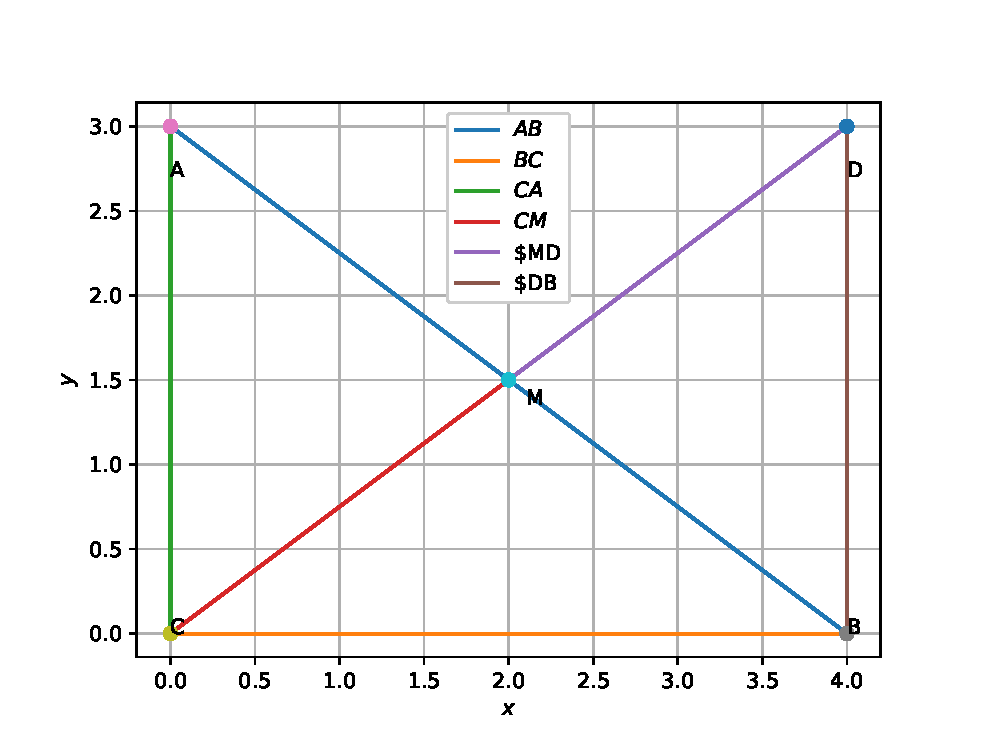
\includegraphics[scale=0.275]{./figs/triangle.eps}
\caption{\tiny By Python}
\end{subfigure}
%
\begin{subfigure}{0.65\textwidth}
\begin{flushright}


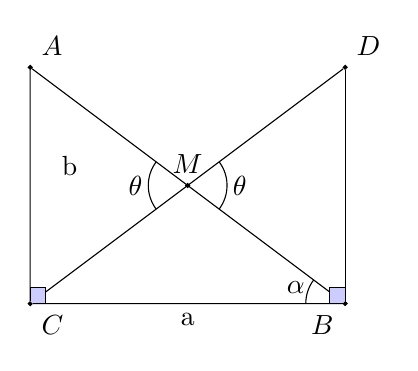
\begin{tikzpicture}
[scale=1,>=stealth,point/.style={draw,circle,fill = black,inner sep=0.5pt},]

%Triangle sides
\def\a{4}
\def\b{3}
\def\c{sqrt(\a^2+\c^2)}



%Labeling points
\node (A) at (0,\b)[point,label=above right:$A$] {};
\node (B) at (\a, 0)[point,label=below left:$B$] {};
\node (C) at (0, 0)[point,label=below right:$C$] {};
\node (M) at (\a*0.5,\b*0.5)[point,label=above:$M$] {};
\node (D) at (\a,\b)[point,label=above right:$D$] {};


%Drawing triangle ABC
\draw (A) -- node[left] {$\textrm{}$} (B) -- node[below] {$\textrm{a}$} (C) -- node[above,xshift=5mm] {$\textrm{b}$} (A);

%Joining CD
\draw (C)--(D);
%Joining BD
\draw (B)--(D);

%Drawing and marking angles
\tkzMarkAngle[fill=orange!40,size=0.5cm,mark=](A,M,C)
\tkzMarkAngle[fill=orange!40,size=0.5cm,mark=](B,M,D)
\tkzMarkAngle[fill=green!40,size=0.5cm,mark=](A,B,C)
\tkzMarkRightAngle[fill=blue!20,size=.2](A,C,B)
\tkzMarkRightAngle[fill=blue!20,size=.2](D,B,C)
\tkzLabelAngle[pos=0.65](A,M,C){$\theta$}
\tkzLabelAngle[pos=0.65](B,M,D){$\theta$}
\tkzLabelAngle[pos=0.65](A,B,C){$\alpha$}


\end{tikzpicture}

\caption{\tiny By Latex-tikz}
\end{flushright}
\end{subfigure}
\end{flushleft}
%
\end{figure}
\end{frame}
\section*{\textbf{Solution}}
\begin{frame}[fragile]
\frametitle{Solution}
\footnotesize
\label{abcd}
\begin{columns}
\begin{column}{0.5\textwidth}
\textbf{Sol a)}
$\triangle AMC \cong \triangle DMB$  by SAS congruency 
$\because$
\\
$AM = BM$
\\
$CM = DM$
\\
$\angle{AMC} = \angle{DMB}( Vertically Opposite Angles)$
\\
\textbf{Sol c)}
\begin{align}
\norm{\vec{A}-\vec{B}} &= \norm{\myvec{-a \\ b}}
\\
\norm{\vec{C}-\vec{D}} &= \norm{\myvec{-a \\ -b}}
\\
\implies \norm{\vec{A}-\vec{B}} &= \norm{\vec{C}-\vec{D}}\\
\label{eq:solution_c}
\text{or, } AB &=CD
\end{align}
From RHS congruence,  $\triangle ACB \cong  \triangle DCB$
\end{column}
\begin{column}{0.5\textwidth}
\textbf{Sol b)}
From \eqref{eq:constr_b}, \eqref{eq:constr_c}, \eqref{eq:constr_d}
\begin{align}
\brak{\vec{D}-\vec{B}}^T
\brak{\vec{B}-\vec{C}} &= \myvec{0 & b}\myvec{a \\ 0} = 0
\\
\implies BD \perp BC
\end{align}
\textbf{Sol d)}
From \eqref{eq:solution_c}, noting that $\vec{M}$ is the mid point of both $AB$ and $CD$, 
\begin{align}
\norm{\vec{A}-\vec{B}} &= \norm{\myvec{-a \\ b}}
\\
\norm{\vec{C}-\vec{D}} &= \norm{\myvec{-a \\ -b}}
\\
\implies \norm{\vec{A}-\vec{B}} &= \norm{\vec{C}-\vec{D}}\\
\text{or, } AB &=CD
\end{align}
\end{column}
\end{columns}
\end{frame}




\end{document}